\documentclass[11pt]{article}
\usepackage{geometry}
\usepackage{amsmath}
\usepackage{amssymb}
\usepackage{enumitem}
\usepackage{fancyhdr}
\usepackage{palatino}
\usepackage{tikz}
\usepackage{tcolorbox}

\usetikzlibrary{trees}
\pagestyle{fancy}

\lhead{MTH 201}
\chead{Derivatives of inverse functions and implicit functions}
\rhead{2018-10-15}

\begin{document}

\begin{center}
    \Large{Practice: Derivatives of inverse functions and implicit functions}
\end{center}

\subsection*{Warmup}

Write down the derivative formulas: 

\begin{align*}
    \frac{d}{dx}\left[\ln(x) \right] &= \hspace{2in} \\
    \frac{d}{dx}\left[\arcsin(x) \right] &= \hspace{2in} \\
    \frac{d}{dx}\left[\arctan(x) \right] &= \hspace{2in}
\end{align*}


\subsection*{Derivatives of inverse functions}

Find the derivative of each of the following. Check your work with Wolfram Alpha. DO NOT try to simplify algebra or trig for now. Six of these will go on the board. The remaining ones will be posted on Slack. 

\begin{enumerate}
    \item $h(x) = x^2 \ln(x)$
    \item $j(x) = \ln(x^2 + 1)$
    \item $k(w) = \arcsin(x^3 + x^2 + x + 1)$
    \item $p(t) = \dfrac{\ln(t)}{e^t + 1}$
    \item $m(z) = \ln(\ln(z))$
    \item $s(y) = \ln(\cos(y) + 2)$
    \item $z(x) = \tan(\ln(x))$
    \item $m(v) = \ln(\sin^2(v) + 1)$
    \item $j(r) = \arctan(e^r + \ln(r))$
    \item $s(y) = \cot(\arctan(y))$
\end{enumerate}

\vspace

\subsection*{Tangent lines to curves}

Consider the curve traced out by the equation $x^3 - y^3 = 6xy$ and look at the point $(-3,3)$ that sits on this curve. 

\begin{center}
    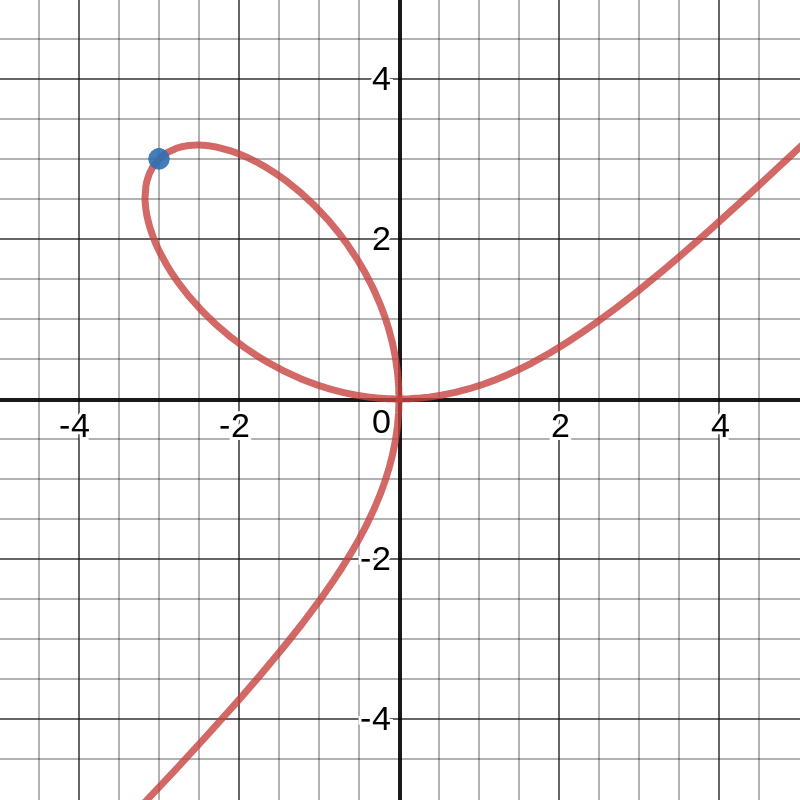
\includegraphics[width=3in]{implicit-curve.png}}
\end{center}
Find a formula for the tangent line to the curve at this point. Follow these steps: 
\begin{enumerate}
    \item First, before calculating anything, draw the tangent line yourself and estimate its slope and $y$-intercept.
    \item Find $dy/dx$ in terms of $x$ and $y$ using the implicit differentiation technique studied in the Guided Inquiry. 
    \item Use the point given to find the slope of the tangent line at that point. 
    \item Then use the point-slope form for the equation of a line to get the tangent line. (Google terms if needed.) 
    \item Check your calculus work against the estimations you made in the first step. If they are way off from each other, double-check your calculus. 
\end{enumerate}


\end{document}